\documentclass[12pt]{article}
\usepackage[framemethod=TikZ]{mdframed}
\usepackage{amsthm}
\usepackage{tcolorbox}
\usepackage[legalpaper, margin=0.75in]{geometry}
\usepackage{setspace}
\usepackage{amsmath}
\usepackage{cancel}
\usepackage{multicol}
\def\deg{\ensuremath{^\circ}}
\def\v#1{\ensuremath{\mathrm{#1}}}
\usepackage{multirow}
\usepackage{fancyhdr}
\pagestyle{fancy}
\usepackage{lastpage} 
\usepackage{colortbl}
\usepackage{amssymb}
\usepackage{graphicx}
\setlength{\parskip}{0pt}
\lhead{Jhon Christian N. Rozano}
\chead{}
\rhead{May 19, 2021}

\lfoot{Source: Brilliant}
\cfoot{}
\rfoot{Page \thepage\ of \pageref{LastPage}}

\renewcommand{\headrulewidth}{1pt}

\renewcommand{\footrulewidth}{1pt}

\newcommand*\Eval[3]{\left.#1\right\rvert_{#2}^{#3}}

\definecolor{LightCyan}{rgb}{0.88,1,1}



\begin{document}
	\setlength{\columnsep}{10pt}
	\renewcommand{\arraystretch}{1.5}
	\singlespacing
	\newtcolorbox{mybox}[1]{title=#1}
	
	\begin{center}
		{\large  \textbf{Physics Problems of the Day}} \\ 
	\end{center}
	\begin{center}
		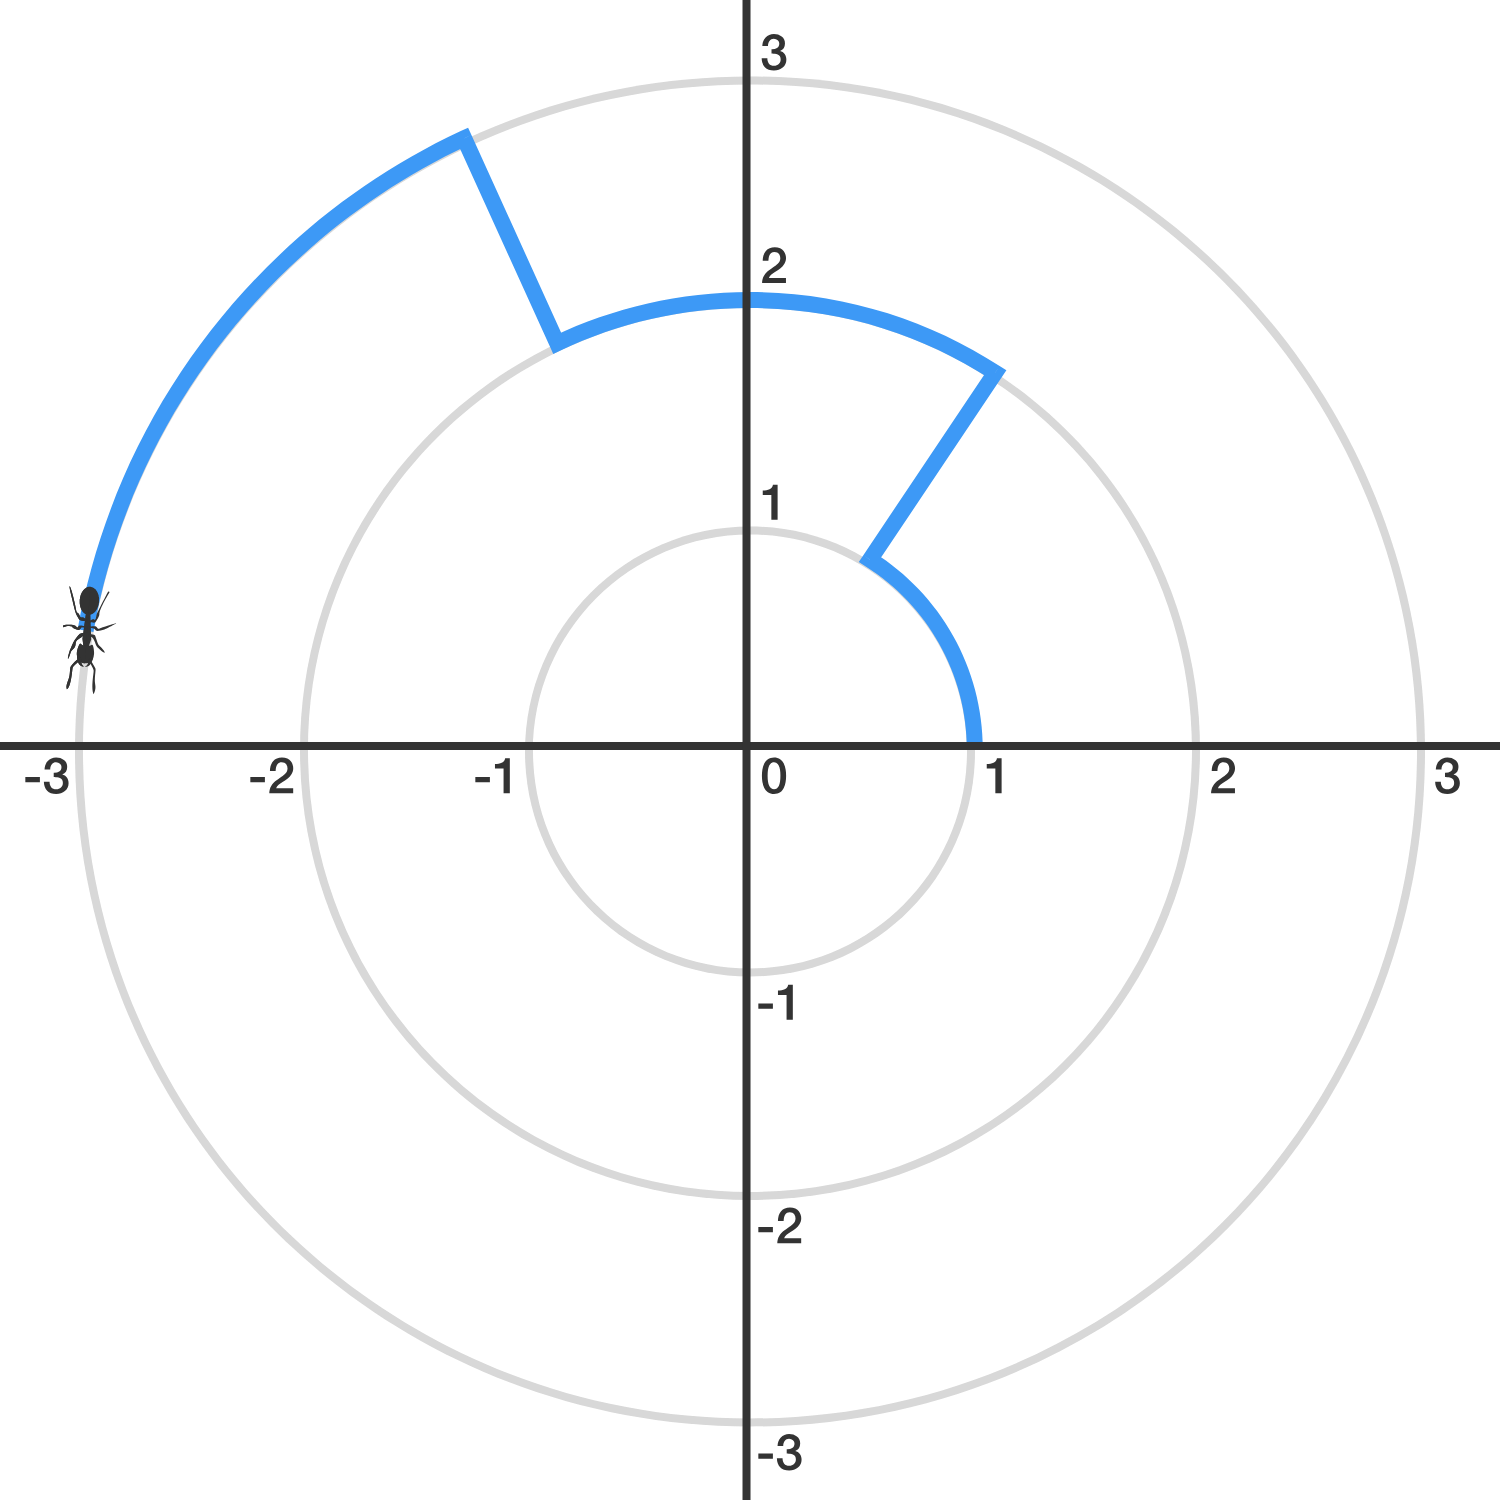
\includegraphics[clip=true, scale=0.09]{ZxY15EJaoO-10708 (1).png}
	\end{center}

	\noindent \textbf{Problem 1:}  An ant finds itself in the \( xy \)-plane, and its initial position is \( (1,0) \). \\
	
	\noindent Let $S_k$ denote the circle with radius $k$ centered around the origin. Starting from \( (1,0) \), the ant walks 1 unit counter-clockwise on $S_1$. Then, it walks directly (radially outward) to $S_2$, on which it will walk 2 units counter-clockwise. Then, it will walk directly to $S_3$ and walk 3 units counter-clockwise, and so, with the ant walking $k$ units on $S_k$. \\
	
	\noindent When the ant crosses the positive $x\text{-axis}$ for the first time since it left \( (1,0) \), it is on $S_n$. What is $n$? \\
	
	\begin{mybox}{\textbf{Solution}}
		Note that the formula for angular position is \( \displaystyle{\theta = \frac{s}{r}} \) where $s$ is the length by which the ant sweeps out and $r$ is the radius. \\
		
		In $S_1, S_2, \text{and}, S_3$, the ant always travels \( \theta = \displaystyle{\frac{s}{r}} = \frac{1}{1} = \frac{2}{2} = \frac{3}{3} = 1\text{ radian} \). The circle extends for about $2\pi\text{ rad} \approx 6.28\text{ rad}$. Hence, after $S_6$, the ant will cross the positive $x\text{-axis}$ for the first time. Therefore, the answer is $S_7$, $\boxed{\textcolor{red}{n=7}}$
	\end{mybox}

	\bigskip
	
	\noindent \textbf{Problem 2:} At the playground, there is a merry-go-round initially at rest, whose moment of inertia is $1320\text{ kg} \cdot \text{m}^2$. A boy weighing $33\text{ kg}$ stands on it, and his distance from the center of the merry-go-round is $8\text{ meters}$. If the boy begins to run in a circular path (about the center of the merry-go-round) with a speed of $6.0\text{ m/s}$ relative to the ground, what is the angular speed of the merry-go-round? \\
	
	\noindent Ignore any friction other than that between the surface of the merry-go-round and the boy. \\
	
	\begin{mybox}{\textbf{Solution}}
		In this problem, the angular momentum of the boy and merry-go-round is conserved throughout. Since the boy only stands on it before running, the initial angular momentum of the system is zero. Therefore, 
		\[ \Delta p = 0 \Rightarrow  p_f = p_i \Rightarrow I_m\omega_m + I_b\omega_b = 0 \]
		where $I_m$, $\omega_m$ is the moment of inertia and the mass of the merry-go-round, and $I_b$, $\omega_b$ is those of the boy.\\
		
		The angular velocity of the boy is given by $\displaystyle{\omega_b = \frac{v}{r} = \frac{6.0\text{ m/s}}{8\text{ m}} = \frac{3}{4}\text{ rad/s}} $. Therefore,
		\[
			I_m\omega_m + I_b\omega_b = 0 \Rightarrow \omega_m = -\frac{I_b}{I_m} \omega_b = - \frac{m_b\cdot{r_b}^2}{I_m}\omega_b
		\]
		\[
			\omega_m = - \frac{ (33\text{ kg})\cdot (8\text{ m})^2 }{1320\text{ kg} \cdot \text{m}^2} \times \frac{3}{4}\text{ rad/s} \approx -1.2\text{ rad/s} 
		\]  
		\noindent Therefore, the magnitude of the angular speed of the merry-go-round is $\boxed{\textcolor{red}{1.2\text{ rad/s}}}.$
	\end{mybox}
	%

\end{document}
